\documentclass[tikz, border=15pt]{standalone}
\usepackage[utf8]{inputenc}
\usepackage{amsmath}
\usetikzlibrary{arrows.meta}

\begin{document}

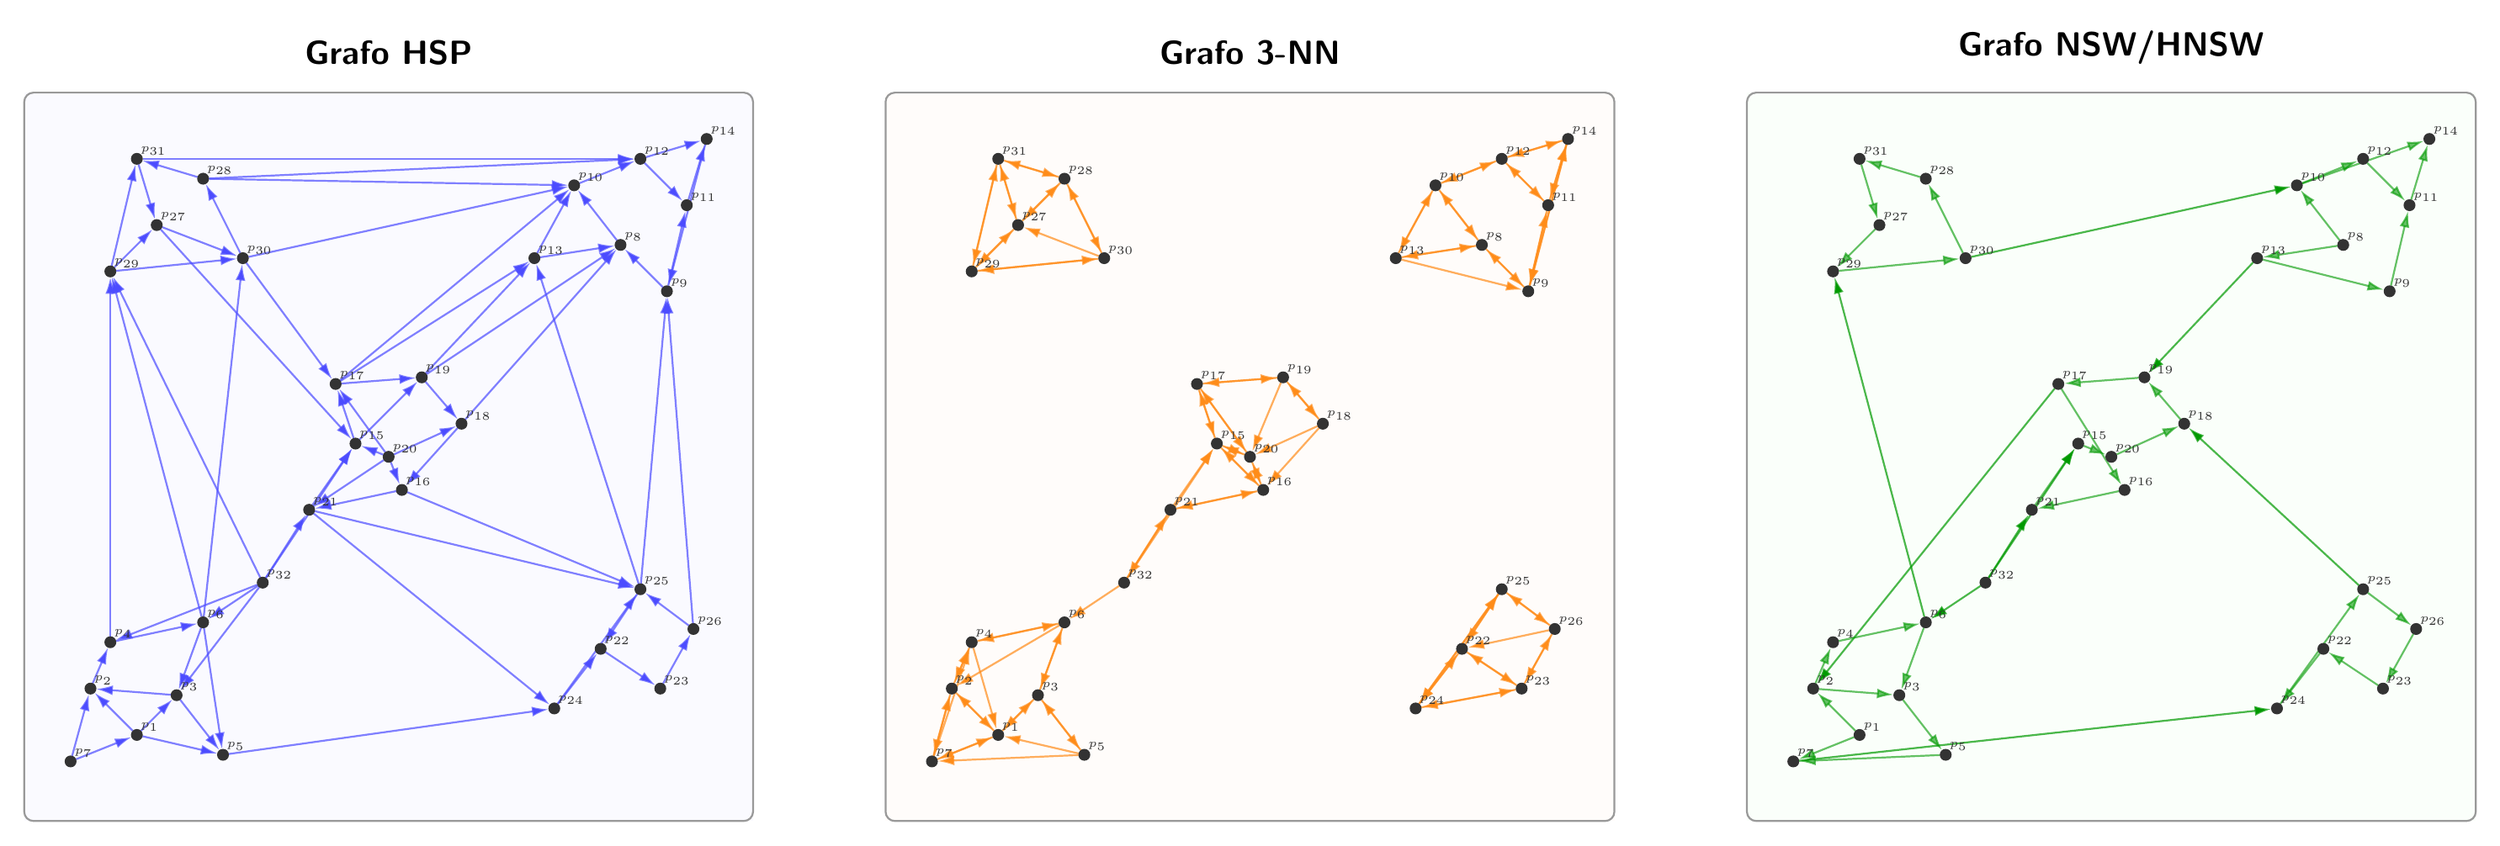
\begin{tikzpicture}[
    font=\sffamily,
    % Estilo de los nodos (32 puntos)
    pnode/.style={circle, fill=black!80, inner sep=1.8pt},
    % Estilo de las aristas HSP (conectividad global dirigida)
    hspedge/.style={thick, blue!70, draw opacity=0.7, -{Latex[length=2.5mm, width=1.5mm]}, shorten >= 2.5pt, shorten <= 2.5pt},
    % Estilo de las aristas 3-NN (asimetría de vecindad local)
    knnedge/.style={thick, orange!90, draw opacity=0.7, -{Latex[length=2.5mm, width=1.5mm]}, shorten >= 2.5pt, shorten <= 2.5pt},
    % Estilo de las aristas NSW (Mundo Pequeño)
    nswedge/.style={thick, green!60!black, draw opacity=0.7, -{Latex[length=2.5mm, width=1.5mm]}, shorten >= 2.5pt, shorten <= 2.5pt},
    % Estilo para la inserción del i-ésimo nodo
    iedge/.style={very thick, red, dashed, -{Latex[length=2.5mm, width=2mm]}, shorten >= 2.5pt, shorten <= 2.5pt},
    % Estilo de las cajas contenedoras
    box/.style={thick, draw=black!40, rounded corners=4pt}
]

% ==========================================
% DEFINICIÓN DE LOS 32 PUNTOS (MACRO COMPARTIDA)
% ==========================================
\newcommand{\setcoords}{
    % Clúster 1: Inferior Izquierdo (7 puntos)
    \coordinate (p1) at (1.2, 0.8);
    \coordinate (p2) at (0.5, 1.5);
    \coordinate (p3) at (1.8, 1.4);
    \coordinate (p4) at (0.8, 2.2);
    \coordinate (p5) at (2.5, 0.5);
    \coordinate (p6) at (2.2, 2.5);
    \coordinate (p7) at (0.2, 0.4);

    % Clúster 2: Superior Derecho (7 puntos)
    \coordinate (p8) at (8.5, 8.2);
    \coordinate (p9) at (9.2, 7.5);
    \coordinate (p10) at (7.8, 9.1);
    \coordinate (p11) at (9.5, 8.8);
    \coordinate (p12) at (8.8, 9.5);
    \coordinate (p13) at (7.2, 8.0);
    \coordinate (p14) at (9.8, 9.8);

    % Clúster 3: Centro (7 puntos)
    \coordinate (p15) at (4.5, 5.2);
    \coordinate (p16) at (5.2, 4.5);
    \coordinate (p17) at (4.2, 6.1);
    \coordinate (p18) at (6.1, 5.5);
    \coordinate (p19) at (5.5, 6.2);
    \coordinate (p20) at (5.0, 5.0);
    \coordinate (p21) at (3.8, 4.2);

    % Clúster 4: Inferior Derecho (5 puntos)
    \coordinate (p22) at (8.2, 2.1);
    \coordinate (p23) at (9.1, 1.5);
    \coordinate (p24) at (7.5, 1.2);
    \coordinate (p25) at (8.8, 3.0);
    \coordinate (p26) at (9.6, 2.4);

    % Clúster 5: Superior Izquierdo (5 puntos)
    \coordinate (p27) at (1.5, 8.5);
    \coordinate (p28) at (2.2, 9.2);
    \coordinate (p29) at (0.8, 7.8);
    \coordinate (p30) at (2.8, 8.0);
    \coordinate (p31) at (1.2, 9.5);

    % Nodo 32: Puente estratégico / i-ésimo punto
    \coordinate (p32) at (3.1, 3.1);
}

% Macro para dibujar los nodos y asignarles su leyenda pi automáticamente
\newcommand{\drawnodes}{
    \foreach \i in {1,...,32} {
        \node[pnode] at (p\i) {};
        \node[font=\tiny, text=black!80, anchor=south west, inner sep=1.5pt] at (p\i) {$p_{\i}$};
    }
}

% ==========================================
% CUADRO 1: GRAFO HSP (Half-Space Partitioning)
% ==========================================
\begin{scope}[shift={(0,0)}]
    % Fondo suave
    \fill[blue!2] (-0.5, -0.5) rectangle (10.5, 10.5);
    \draw[box] (-0.5, -0.5) rectangle (10.5, 10.5);
    
    % Aseguramos que las coordenadas existan antes de trazar aristas
    \setcoords
    
    % Aristas internas de los clústeres (Malla base)
    \path[hspedge] (p7) edge (p1) (p7) edge (p2) (p1) edge (p2) (p1) edge (p5) (p2) edge (p4) (p4) edge (p6) (p6) edge (p3) (p3) edge (p2) (p1) edge (p3) (p3) edge (p5) (p6) edge (p5);
    \path[hspedge] (p13) edge (p8) (p8) edge (p10) (p10) edge (p12) (p12) edge (p11) (p11) edge (p14) (p14) edge (p9) (p9) edge (p11) (p9) edge (p8) (p12) edge (p14) (p13) edge (p10);
    \path[hspedge] (p20) edge (p15) (p20) edge (p16) (p20) edge (p17) (p20) edge (p18) (p20) edge (p21) (p15) edge (p17) (p17) edge (p19) (p19) edge (p18) (p18) edge (p16) (p16) edge (p21) (p21) edge (p15) (p15) edge (p19);
    \path[hspedge] (p24) edge (p22) (p22) edge (p23) (p23) edge (p26) (p26) edge (p25) (p25) edge (p22) (p24) edge (p25);
    \path[hspedge] (p29) edge (p27) (p27) edge (p30) (p30) edge (p28) (p28) edge (p31) (p31) edge (p27) (p29) edge (p31) (p29) edge (p30);
    
    % Aristas HSP INTER-CLÚSTER (Conectividad Global gracias a evitar sombras)
    \path[hspedge] (p5) edge (p24); % Base C1-C4
    \path[hspedge] (p4) edge (p29); % Borde C1-C5
    \path[hspedge] (p6) edge (p29) (p6) edge (p30); % Borde C1-C5 interno
    \path[hspedge] (p32) edge (p6) (p32) edge (p3) (p32) edge (p21) (p32) edge (p15) (p32) edge (p4) (p32) edge (p29); % Conexiones del puente
    \path[hspedge] (p21) edge (p24) (p21) edge (p25) (p16) edge (p25); % C3 a C4
    \path[hspedge] (p26) edge (p9) (p25) edge (p9) (p25) edge (p13); % C4 a C2
    \path[hspedge] (p18) edge (p8) (p19) edge (p8) (p19) edge (p13) (p17) edge (p13) (p17) edge (p10); % C3 a C2
    \path[hspedge] (p30) edge (p17) (p27) edge (p15); % C5 a C3
    \path[hspedge] (p30) edge (p10) (p28) edge (p10) (p31) edge (p12) (p28) edge (p12); % C5 a C2
    
    \drawnodes
    
    % Etiquetas
    \node[anchor=south] at (5, 10.8) {\Large \textbf{Grafo HSP}};
    %\node[anchor=north, text width=9.5cm, align=center] at (5, -0.8) {
    %    \textbf{Conectividad Global Garantizada:} Al descartar únicamente los medios espacios, se crea una malla continua. Las flechas indican qué nodos expanden la búsqueda hacia otras regiones sin mínimos locales asilados.
    %};
\end{scope}

% ==========================================
% CUADRO 2: GRAFO 3-NN (k-Nearest Neighbors)
% ==========================================
\begin{scope}[shift={(13,0)}]
    % Fondo suave
    \fill[orange!2] (-0.5, -0.5) rectangle (10.5, 10.5);
    \draw[box] (-0.5, -0.5) rectangle (10.5, 10.5);
    
    \setcoords
    
    % Aristas 3-NN dirigidas: Cálculo riguroso (exactamente 3 aristas salientes por nodo)
    % Las opacidades (0.7) permiten ver las aristas bidireccionales superpuestas
    
    % Clúster 1
    \path[knnedge] (p1) edge (p2) (p1) edge (p3) (p1) edge (p7);
    \path[knnedge] (p2) edge (p1) (p2) edge (p4) (p2) edge (p7);
    \path[knnedge] (p3) edge (p1) (p3) edge (p5) (p3) edge (p6);
    \path[knnedge] (p4) edge (p2) (p4) edge (p6) (p4) edge (p1);
    \path[knnedge] (p5) edge (p1) (p5) edge (p3) (p5) edge (p7);
    \path[knnedge] (p6) edge (p3) (p6) edge (p4) (p6) edge (p2);
    \path[knnedge] (p7) edge (p1) (p7) edge (p2) (p7) edge (p4);
    
    % Clúster 2
    \path[knnedge] (p8) edge (p10) (p8) edge (p13) (p8) edge (p9);
    \path[knnedge] (p9) edge (p8) (p9) edge (p11) (p9) edge (p14);
    \path[knnedge] (p10) edge (p8) (p10) edge (p12) (p10) edge (p13);
    \path[knnedge] (p11) edge (p9) (p11) edge (p12) (p11) edge (p14);
    \path[knnedge] (p12) edge (p10) (p12) edge (p11) (p12) edge (p14);
    \path[knnedge] (p13) edge (p8) (p13) edge (p10) (p13) edge (p9);
    \path[knnedge] (p14) edge (p11) (p14) edge (p12) (p14) edge (p9);
    
    % Clúster 3 + Nodo Puente p32
    \path[knnedge] (p15) edge (p16) (p15) edge (p20) (p15) edge (p17);
    \path[knnedge] (p16) edge (p15) (p16) edge (p20) (p16) edge (p21);
    \path[knnedge] (p17) edge (p15) (p17) edge (p19) (p17) edge (p20);
    \path[knnedge] (p18) edge (p19) (p18) edge (p16) (p18) edge (p20);
    \path[knnedge] (p19) edge (p17) (p19) edge (p18) (p19) edge (p20);
    \path[knnedge] (p20) edge (p15) (p20) edge (p16) (p20) edge (p17);
    \path[knnedge] (p21) edge (p15) (p21) edge (p16) (p21) edge (p32);
    \path[knnedge] (p32) edge (p21) (p32) edge (p6) (p32) edge (p15);
    
    % Clúster 4
    \path[knnedge] (p22) edge (p24) (p22) edge (p23) (p22) edge (p25);
    \path[knnedge] (p23) edge (p22) (p23) edge (p24) (p23) edge (p26);
    \path[knnedge] (p24) edge (p22) (p24) edge (p23) (p24) edge (p25);
    \path[knnedge] (p25) edge (p26) (p25) edge (p22) (p25) edge (p24);
    \path[knnedge] (p26) edge (p23) (p26) edge (p25) (p26) edge (p22);
    
    % Clúster 5
    \path[knnedge] (p27) edge (p29) (p27) edge (p28) (p27) edge (p31);
    \path[knnedge] (p28) edge (p27) (p28) edge (p30) (p28) edge (p31);
    \path[knnedge] (p29) edge (p27) (p29) edge (p30) (p29) edge (p31);
    \path[knnedge] (p30) edge (p28) (p30) edge (p29) (p30) edge (p27);
    \path[knnedge] (p31) edge (p28) (p31) edge (p27) (p31) edge (p29);
    
    \drawnodes
    
    % Etiquetas
    \node[anchor=south] at (5, 10.8) {\Large \textbf{Grafo 3-NN}};
    %\node[anchor=north, text width=9.5cm, align=center] at (5, -0.8) {    \textbf{Fragmentación y Asimetría:} al forzar conexiones solo con los $k=3$ más cercanos, el espacio se fragmenta en islas desconectadas.};
\end{scope}

% ==========================================
% CUADRO 3: GRAFO NSW/HNSW (Construcción Incremental)
% ==========================================
\begin{scope}[shift={(26,0)}]
    % Fondo suave
    \fill[green!2] (-0.5, -0.5) rectangle (10.5, 10.5);
    \draw[box] (-0.5, -0.5) rectangle (10.5, 10.5);
    
    \setcoords
    
    % 1. Enlaces cortos dirigidos (Nodos insertados tardíamente)
    \path[nswedge, opacity=0.6] (p1) edge (p2) (p1) edge (p7) (p2) edge (p4) (p4) edge (p6) (p6) edge (p3) (p3) edge (p5) (p5) edge (p7) (p2) edge (p3);
    \path[nswedge, opacity=0.6] (p8) edge (p10) (p10) edge (p12) (p12) edge (p11) (p11) edge (p14) (p9) edge (p11) (p8) edge (p13) (p13) edge (p9) (p10) edge (p14);
    \path[nswedge, opacity=0.6] (p15) edge (p20) (p20) edge (p18) (p18) edge (p19) (p19) edge (p17) (p17) edge (p16) (p16) edge (p21) (p21) edge (p15);
    \path[nswedge, opacity=0.6] (p22) edge (p24) (p24) edge (p25) (p25) edge (p26) (p26) edge (p23) (p23) edge (p22);
    \path[nswedge, opacity=0.6] (p27) edge (p29) (p29) edge (p30) (p30) edge (p28) (p28) edge (p31) (p31) edge (p27);
    
    % 2. "Atajos" o Long-range links (sin etiqueta explícita de atajo antiguo)
    \path[nswedge, thick] (p7) edge (p24); 
    \path[nswedge, thick] (p6) edge (p29);
    \path[nswedge, thick] (p30) edge (p10);
    \path[nswedge, thick] (p13) edge (p19);
    \path[nswedge, thick] (p25) edge (p18);
    \path[nswedge, thick] (p17) edge (p2);
    
    % 3. El i-ésimo punto (Inserción de p32). 
    % Trazamos las líneas y radio primero para no sobreescribir los nodos.
    %\draw[red, thick, dotted] (p32) circle (1.45cm);
    
    % Conectando p32 a sus M=3 vecinos (las flechas rojas muestran la inserción en tiempo real)
    \path[nswedge] (p32) edge (p6);
    \path[nswedge] (p32) edge (p21);
    \path[nswedge] (p32) edge (p15);
    
    % Dibujamos todos los nodos uniformemente (incluido p32)
    \drawnodes
    
    % Etiquetas
    \node[anchor=south] at (5, 10.8) {\Large \textbf{Grafo NSW/HNSW}};
    %\node[anchor=north, text width=9.5cm, align=center] at (5, -0.8) {
    %    \textbf{Construcción Incremental Dirigida:} Al llegar el nodo $p_{32}$.
    %};
\end{scope}

\end{tikzpicture}

\end{document}
